\documentclass{article}
\usepackage{amsmath}
\usepackage{color,pxfonts,fix-cm}
\usepackage{latexsym}
\usepackage[mathletters]{ucs}
\DeclareUnicodeCharacter{46}{\textperiodcentered}
\DeclareUnicodeCharacter{60}{\textless}
\DeclareUnicodeCharacter{62}{\textgreater}
\DeclareUnicodeCharacter{32}{$\ $}
\usepackage[T1]{fontenc}
\usepackage[utf8x]{inputenc}
\usepackage{pict2e}
\usepackage{wasysym}
\usepackage[english]{babel}
\usepackage{tikz}
\pagestyle{empty}
\usepackage[margin=0in,paperwidth=595pt,paperheight=841pt]{geometry}
\begin{document}
\definecolor{color_29791}{rgb}{0,0,0}
\begin{tikzpicture}[overlay]\path(0pt,0pt);\end{tikzpicture}
\begin{picture}(-5,0)(2.5,0)
\put(70.104,-64.67999){\fontsize{20.04}{1}\usefont{T2A}{cmr}{m}{n}\selectfont\color{color_29791}МИНИСТЕРСТВО НАУКИ И ВЫСШЕГО ОБРАЗОВАНИЯ }
\put(70.104,-89.17999){\fontsize{20.04}{1}\usefont{T1}{cmr}{m}{n}\selectfont\color{color_29791}                     РОССИЙСКОЙ ФЕДЕРАЦИИ }
\put(70.104,-107.9){\fontsize{14.04}{1}\usefont{T2A}{cmr}{m}{n}\selectfont\color{color_29791}Федеральное государственное бюджетное образовательное учреждение }
\put(70.104,-125.06){\fontsize{14.04}{1}\usefont{T1}{cmr}{m}{n}\selectfont\color{color_29791}                                           высшего образования }
\put(70.104,-147.74){\fontsize{20.04}{1}\usefont{T2A}{cmr}{b}{n}\selectfont\color{color_29791}АДЫГЕЙСКИЙ ГОСУДАРСТВЕННЫЙ УНИВЕРСИТЕТ }
\put(70.104,-166.58){\fontsize{20.04}{1}\usefont{T1}{cmr}{b}{n}\selectfont\color{color_29791}                        Инженерно-физический факультет }
\put(70.104,-183.62){\fontsize{14.04}{1}\usefont{T1}{cmr}{m}{n}\selectfont\color{color_29791}    Кафедра автоматизированных систем обработки информации и }
\put(70.104,-200.78){\fontsize{14.04}{1}\usefont{T1}{cmr}{m}{n}\selectfont\color{color_29791}                                                      управления }
\put(70.104,-223.46){\fontsize{20.04}{1}\usefont{T1}{cmr}{b}{n}\selectfont\color{color_29791} }
\put(70.104,-247.82){\fontsize{20.04}{1}\usefont{T1}{cmr}{b}{n}\selectfont\color{color_29791} }
\put(70.104,-272.33){\fontsize{20.04}{1}\usefont{T1}{cmr}{b}{n}\selectfont\color{color_29791} }
\put(70.104,-296.69){\fontsize{20.04}{1}\usefont{T1}{cmr}{b}{n}\selectfont\color{color_29791} }
\put(70.104,-321.17){\fontsize{20.04}{1}\usefont{T1}{cmr}{b}{n}\selectfont\color{color_29791} }
\put(70.104,-345.53){\fontsize{20.04}{1}\usefont{T1}{cmr}{b}{n}\selectfont\color{color_29791}                             Отчёт по практике  }
\put(70.104,-370.01){\fontsize{14.04}{1}\usefont{T1}{cmr}{m}{n}\selectfont\color{color_29791}                                                     Вариант 7 }
\put(70.104,-394.37){\fontsize{14.04}{1}\usefont{T1}{cmr}{m}{n}\selectfont\color{color_29791}                          Найти определитель матрицы. }
\put(70.104,-418.85){\fontsize{20.04}{1}\usefont{T1}{cmr}{m}{n}\selectfont\color{color_29791}                      1 курс, группа ИВТ АСОИУ }
\put(70.104,-443.23){\fontsize{20.04}{1}\usefont{T1}{cmr}{m}{n}\selectfont\color{color_29791} }
\put(70.104,-467.59){\fontsize{20.04}{1}\usefont{T1}{cmr}{m}{n}\selectfont\color{color_29791} }
\put(70.104,-492.07){\fontsize{20.04}{1}\usefont{T1}{cmr}{m}{n}\selectfont\color{color_29791} }
\put(70.104,-516.43){\fontsize{20.04}{1}\usefont{T1}{cmr}{m}{n}\selectfont\color{color_29791} }
\put(70.104,-540.91){\fontsize{20.04}{1}\usefont{T1}{cmr}{m}{n}\selectfont\color{color_29791} }
\put(70.104,-559.63){\fontsize{14.04}{1}\usefont{T1}{cmr}{m}{n}\selectfont\color{color_29791}                                                                          Выполнил:  }
\put(70.104,-576.79){\fontsize{14.04}{1}\usefont{T1}{cmr}{m}{n}\selectfont\color{color_29791}                                                                          \_\_\_\_\_\_\_\_\_\_\_\_\_\_\_\_\_\_\_ К.В. Рябенко }
\put(70.104,-593.83){\fontsize{14.04}{1}\usefont{T1}{cmr}{m}{n}\selectfont\color{color_29791}                                                                          «\_\_\_\_\_»\_\_\_\_\_\_\_\_\_\_\_\_ 2024 г. }
\put(70.104,-610.9){\fontsize{14.04}{1}\usefont{T1}{cmr}{m}{n}\selectfont\color{color_29791}                                                                          Руководитель: }
\put(70.104,-628.06){\fontsize{14.04}{1}\usefont{T1}{cmr}{m}{n}\selectfont\color{color_29791}                                                                          \_\_\_\_\_\_\_\_\_\_\_\_\_\_\_\_\_\_\_ С.В. Теплоухов }
\put(70.104,-645.1){\fontsize{14.04}{1}\usefont{T1}{cmr}{m}{n}\selectfont\color{color_29791}                                                                          «\_\_\_\_\_»\_\_\_\_\_\_\_\_\_\_\_\_ 2024 г. }
\put(70.104,-662.26){\fontsize{14.04}{1}\usefont{T1}{cmr}{m}{n}\selectfont\color{color_29791}   }
\put(70.104,-679.3){\fontsize{14.04}{1}\usefont{T1}{cmr}{m}{n}\selectfont\color{color_29791} }
\put(70.104,-696.46){\fontsize{14.04}{1}\usefont{T1}{cmr}{m}{n}\selectfont\color{color_29791} }
\put(70.104,-713.5){\fontsize{14.04}{1}\usefont{T1}{cmr}{m}{n}\selectfont\color{color_29791} }
\put(70.104,-730.54){\fontsize{14.04}{1}\usefont{T1}{cmr}{m}{n}\selectfont\color{color_29791} }
\put(70.104,-747.696){\fontsize{14.04}{1}\usefont{T1}{cmr}{m}{n}\selectfont\color{color_29791} }
\put(70.104,-764.736){\fontsize{14.04}{1}\usefont{T1}{cmr}{m}{n}\selectfont\color{color_29791}                                                        Майкоп 2024 г. }
\end{picture}
\newpage
\begin{tikzpicture}[overlay]\path(0pt,0pt);\end{tikzpicture}
\begin{picture}(-5,0)(2.5,0)
\put(70.104,-64.67999){\fontsize{20.04}{1}\usefont{T2A}{cmr}{m}{n}\selectfont\color{color_29791}СОДЕРЖАНИЕ }
\put(88.1,-89.17999){\fontsize{20.04}{1}\usefont{T1}{cmr}{m}{n}\selectfont\color{color_29791}1) Задача }
\put(88.1,-113.54){\fontsize{20.04}{1}\usefont{T1}{cmr}{m}{n}\selectfont\color{color_29791}2) Пример кода, решающего данную задачу }
\put(88.1,-138.02){\fontsize{20.04}{1}\usefont{T1}{cmr}{m}{n}\selectfont\color{color_29791}3) Скриншот работы программы }
\put(70.104,-162.38){\fontsize{20.04}{1}\usefont{T1}{cmr}{m}{n}\selectfont\color{color_29791} }
\put(70.104,-186.86){\fontsize{20.04}{1}\usefont{T1}{cmr}{m}{n}\selectfont\color{color_29791} }
\put(70.104,-211.22){\fontsize{20.04}{1}\usefont{T1}{cmr}{m}{n}\selectfont\color{color_29791} }
\put(70.104,-235.7){\fontsize{20.04}{1}\usefont{T1}{cmr}{m}{n}\selectfont\color{color_29791} }
\put(70.104,-260.09){\fontsize{20.04}{1}\usefont{T1}{cmr}{b}{n}\selectfont\color{color_29791}1. Задача }
\put(70.104,-284.57){\fontsize{20.04}{1}\usefont{T1}{cmr}{b}{n}\selectfont\color{color_29791}   Найти определитель матрицы. }
\put(70.104,-308.93){\fontsize{20.04}{1}\usefont{T1}{cmr}{m}{n}\selectfont\color{color_29791} }
\put(70.104,-333.29){\fontsize{20.04}{1}\usefont{T1}{cmr}{m}{n}\selectfont\color{color_29791} }
\put(70.104,-357.77){\fontsize{20.04}{1}\usefont{T1}{cmr}{b}{n}\selectfont\color{color_29791}2. Пример кода }
\put(70.104,-374.57){\fontsize{12}{1}\usefont{T1}{cmr}{m}{n}\selectfont\color{color_29791}\#include <iostream> }
\put(70.104,-389.21){\fontsize{12}{1}\usefont{T1}{cmr}{m}{n}\selectfont\color{color_29791} }
\put(70.104,-403.85){\fontsize{12}{1}\usefont{T1}{cmr}{m}{n}\selectfont\color{color_29791}int determinant(int a1, int a2, int a3, int b1, int b2, int b3, int c1, int c2, int c3) \{ }
\put(70.104,-418.61){\fontsize{12}{1}\usefont{T1}{cmr}{m}{n}\selectfont\color{color_29791}    return a1 * (b2 * c3 - b3 * c2) - }
\put(70.104,-433.27){\fontsize{12}{1}\usefont{T1}{cmr}{m}{n}\selectfont\color{color_29791}           a2 * (b1 * c3 - b3 * c1) + }
\put(70.104,-447.91){\fontsize{12}{1}\usefont{T1}{cmr}{m}{n}\selectfont\color{color_29791}           a3 * (b1 * c2 - b2 * c1); }
\put(70.104,-462.55){\fontsize{12}{1}\usefont{T1}{cmr}{m}{n}\selectfont\color{color_29791}\} }
\put(70.104,-477.19){\fontsize{12}{1}\usefont{T1}{cmr}{m}{n}\selectfont\color{color_29791} }
\put(70.104,-491.83){\fontsize{12}{1}\usefont{T1}{cmr}{m}{n}\selectfont\color{color_29791}int main() \{ }
\put(70.104,-506.47){\fontsize{12}{1}\usefont{T1}{cmr}{m}{n}\selectfont\color{color_29791}    int a1 = 1, a2 = 0, a3 = -2; }
\put(70.104,-521.11){\fontsize{12}{1}\usefont{T1}{cmr}{m}{n}\selectfont\color{color_29791}    int b1 = -2, b2 = 4, b3 = 5; }
\put(70.104,-535.75){\fontsize{12}{1}\usefont{T1}{cmr}{m}{n}\selectfont\color{color_29791}    int c1 = 0, c2 = -3, c3 = 1; }
\put(70.104,-550.39){\fontsize{12}{1}\usefont{T1}{cmr}{m}{n}\selectfont\color{color_29791} }
\put(70.104,-565.03){\fontsize{12}{1}\usefont{T1}{cmr}{m}{n}\selectfont\color{color_29791}    int det = determinant(a1, a2, a3, b1, b2, b3, c1, c2, c3); }
\put(70.104,-579.67){\fontsize{12}{1}\usefont{T1}{cmr}{m}{n}\selectfont\color{color_29791} }
\put(70.104,-594.31){\fontsize{12}{1}\usefont{T1}{cmr}{m}{n}\selectfont\color{color_29791}    std::cout << "Определитель матрицы: " << det << std::endl; }
\put(70.104,-608.98){\fontsize{12}{1}\usefont{T1}{cmr}{m}{n}\selectfont\color{color_29791} }
\put(70.104,-623.74){\fontsize{12}{1}\usefont{T1}{cmr}{m}{n}\selectfont\color{color_29791}    return 0; }
\put(70.104,-638.38){\fontsize{12}{1}\usefont{T1}{cmr}{m}{n}\selectfont\color{color_29791}\} }
\put(70.104,-653.02){\fontsize{12}{1}\usefont{T1}{cmr}{m}{n}\selectfont\color{color_29791} }
\put(70.104,-667.66){\fontsize{12}{1}\usefont{T1}{cmr}{m}{n}\selectfont\color{color_29791} }
\put(70.104,-682.3){\fontsize{12}{1}\usefont{T1}{cmr}{m}{n}\selectfont\color{color_29791} }
\put(70.104,-696.94){\fontsize{12}{1}\usefont{T1}{cmr}{m}{n}\selectfont\color{color_29791} }
\put(70.104,-711.58){\fontsize{12}{1}\usefont{T1}{cmr}{m}{n}\selectfont\color{color_29791} }
\put(70.104,-726.22){\fontsize{12}{1}\usefont{T1}{cmr}{m}{n}\selectfont\color{color_29791} }
\put(70.104,-740.856){\fontsize{12}{1}\usefont{T1}{cmr}{m}{n}\selectfont\color{color_29791} }
\put(70.104,-755.496){\fontsize{12}{1}\usefont{T1}{cmr}{m}{n}\selectfont\color{color_29791} }
\put(70.104,-770.136){\fontsize{12}{1}\usefont{T1}{cmr}{m}{n}\selectfont\color{color_29791} }
\end{picture}
\newpage
\begin{tikzpicture}[overlay]\path(0pt,0pt);\end{tikzpicture}
\begin{picture}(-5,0)(2.5,0)
\put(70.104,-64.67999){\fontsize{20.04}{1}\usefont{T1}{cmr}{b}{n}\selectfont\color{color_29791}3. Скриншот работы программы. }
\put(70.104,-81.62){\fontsize{12}{1}\usefont{T1}{cmr}{m}{n}\selectfont\color{color_29791} }
\put(538.18,-368.81){\fontsize{14.04}{1}\usefont{T1}{cmr}{m}{n}\selectfont\color{color_29791} }
\put(70.104,-379.25){\fontsize{11.04}{1}\usefont{T1}{cmr}{m}{n}\selectfont\color{color_29791} }
\put(70.104,-409.49){\fontsize{11.04}{1}\usefont{T1}{cmr}{m}{n}\selectfont\color{color_29791}  }
\put(70.05,-368.74){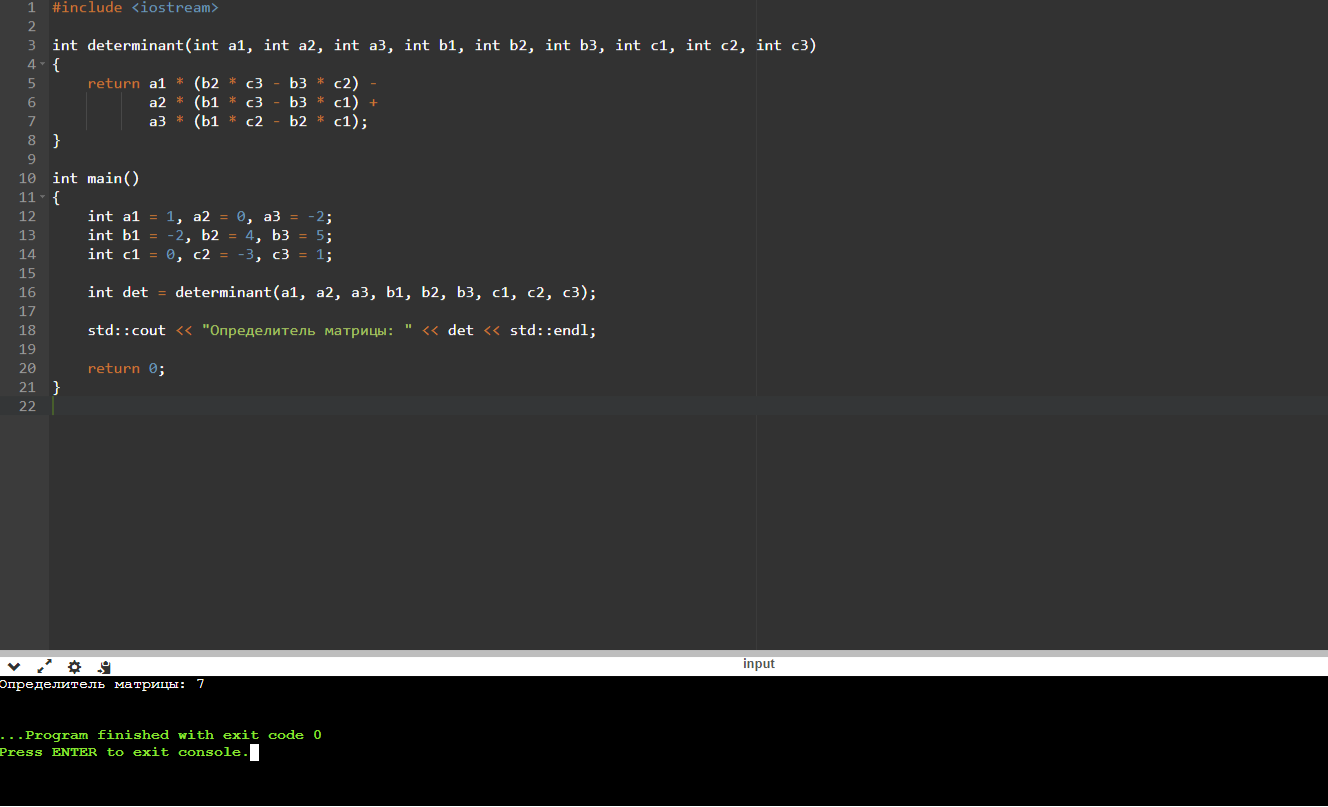
\includegraphics[width=467.3pt,height=283.9pt]{latexImage_3af21e33f25d027c30bc5d8de6ce9cc7.png}}
\end{picture}
\end{document}